\chapter{Introduction}
\todo{Write Introduction}
\section{Background}
\todo[inline]{Write background}
\section{Research Objective}
\todo[inline]{Write Research Objective}
\section{Agile Development}
\todo[inline]{Theory on Agile Development}
\section{Retrospective}
\todo[inline]{Theory and some common techniques for retrospectives, refer to self preproject}
\section{Organizational Learning}
Organizational learning is in simple terms how an organization is able to acquire, store and utilize knowledge existing within an organization. In a more academic setting we can use Argyris and Schön definition \cite{Argyris1996} for organizational learning: 

\begin{quote}
	``Organizational learning occurs when individuals within an organization experience a problematic situation and inquire into it on the organization's behalf. They experience a surprising mismatch between expected and actual results of action and respond to that mismatch through a process of thought and further action that leads them to modify their images of organization or their understandings of organizational phenomena and to restructure their activities so as to bring outcomes and expectation into line, thereby changing organizational theory-in-use. In order to become organizational, the learning that results from organizational inquiry must become embedded in the images of organization held in its members' minds and/or in the epistemological artifacts (the maps, memories, and programs) embedded in the organizational environment. ''
\end{quote}

Organizational learning can be applied to groups of people over different sizes. One can use it to analyze huge organizations consisting of many actors in different roles, or small groups of people working close together. For this research we are going to apply the organizational learning at an agile development team. 

Different types of frameworks exist for organizational learning. Levitt and March uses a framework that see learning in organizations as encoding inferences from history into routines that guide behavior \cite{Levitt1988}. The retrospective is a process of shared learning for an agile development team learning from the last iteration of development. Investigating learning using this framework won't yield much as the retrospective already is seen as a collective learning activity \cite{Dingsoyr2004}. 

Argyris and Schön \cite{Argyris1996} uses two different models to determine how an organization learns through individuals, Model I and Model II. As agile teams often are limited to a close group of individuals we will apply Argyris and Schön's models. To understand these models we first need to investigate two types of learning: Single-loop learning and double-loop learning. Further in this section we will explain these types of learning as well as Model I and Model II. We will also look at Triple-loop learning as it is the concept of learning about learning. 

\subsection{Single-loop}
Single-loop learning is a type of learning defined by Argyris and Schön. It consist of a single-feedback loop that finds an error and a way to fix this problem. Argyris and Schön \cite{Argyris1996} defines single-loop as: 

\begin{quote}
``By single-loop learning we mean instrumental learning that changes strategies of action or assumptions underlying strategies in ways that leave the value of a theory of action unchanged.

... In such learning episodes, a single feed-back loop, mediated by organizational inquiry, connects detected error - that is, an outcome of action mismatched to expectations and, therefore, surprising - to organizational strategies of action and their underlying assumptions. These strategies of action and their underlying assumptions. These strategies or assumptions are modified, in turn, to keep organizational performance within the range set by existing organizational value and norms. The values and norms themselves ... remain unchanged. 
''
\end{quote}

An example of single-loop learning from software development could be finding a bug, find a solution to fix it and the fix it. The single-loop learning would here be learning the solution and fixing the bug. We have provided a basic illustration of single-loop learning in \autoref{figure:single-loop}.

\begin{figure}[!h]
	\centering
	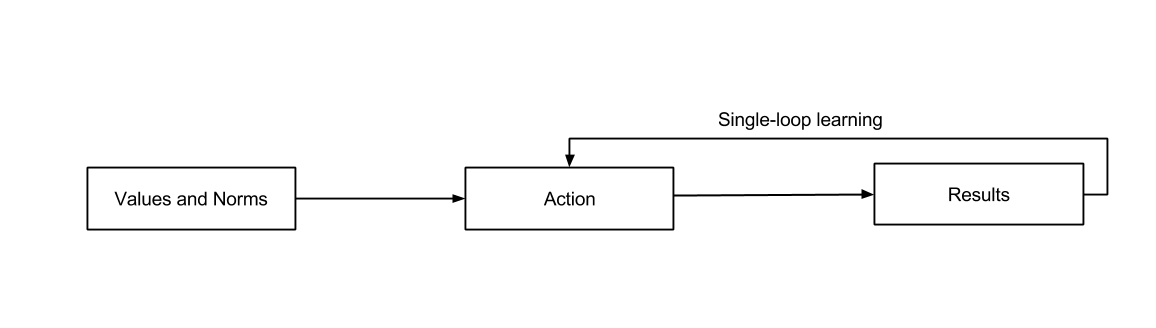
\includegraphics[width=\textwidth, keepaspectratio]{figures/Single-loop.png}
	\caption{Single-loop learning.}
	\label{figure:single-loop}
\end{figure}

\subsection{Double-loop} % (fold)
\label{sub:double_loop}
Double-loop learning is a type of learning where one ask whether the underlying factors that influence the actions and results is sufficient.
One might say that one understand the root-cause for the issue. 
Argyris and Schön defines double-loop learning as: 

\begin{quote}
``By double-loop learning, we mean learning that results in a change in the values of theory-in-use, as well as in its strategies and assumptions. The double loop refers to the two feedback loop that connect the observed effects of actions with startegies and values server by strategies. Strategies and assumptions may change concurrently with, or as a consequence of, change in values. Double-loop learning may be carried out by individuals, when their inquiry leads to change in the values of their theories-in-use or by organizations, when indivduals inquire on behalf of an organization in such a way as to lead to change in the values of organization theory-in-use. ''
\end{quote}

This type of learning can be shown in our bug example. If the developers who earlier found and fixed a bug did a root-cause analysis on the issue they could get several results indicating that underlying factors are not sufficient for the current state of development team. One underlying factor could be weak specification description requiring the team to rethink and restructure how they develop specifications. Another reason could be that the knowledge for the system are not good enough with the developers indicating a knowledge-gap in the team and considerations for the state of the team may be required. 

For this research we use the term double-loop learning when the influences for the issue is understood and change occurs as a results of this. A simple figure of double-loop learning can be seen in \autoref{figure:double-loop}

\begin{figure}[!h]
	\centering
	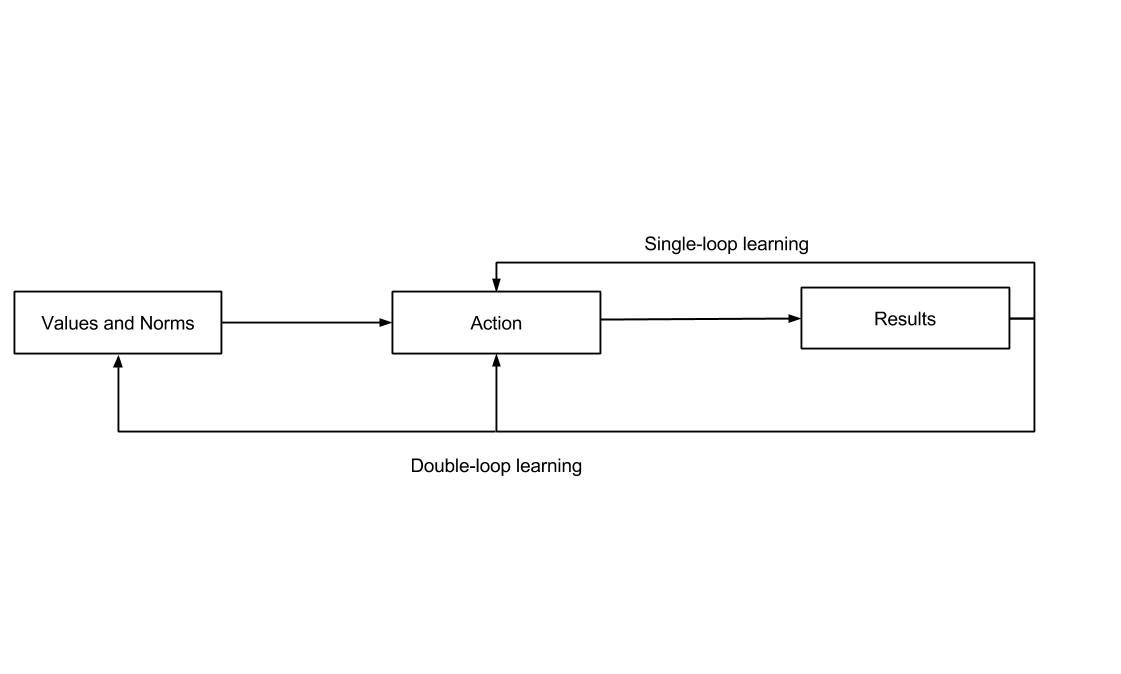
\includegraphics[width=\textwidth, keepaspectratio]{figures/double-loop.png}
	\caption{Double-loop learning.}
	\label{figure:double-loop}
\end{figure}

% subsection triple_loop (end)
\subsection{Model I} % (fold)
\label{sub:model_i}

% subsection model_i (end)
\subsection{Model II} % (fold)
\label{sub:organizational_learning_ii}

% subsection organizational_learning_ii (end)
% subsection double_loop (end)
\subsection{Triple-loop} % (fold)
\label{sub:triple_loop}

\section{Shared Mental Models}

The theory of shared mental models is from cognitive psychology, and can be used as a lens to evaluate agile development and methodology as described by Petter et al\cite{Petter2013}. The concept is that a team has a shared mental model that is central to the mutual understanding between team members, and thus essential to project success. Without a good shared mental model a team is left with a poor understanding of the task at hand, as well as barriers for cooperation. Two metrics used to measure a team's shared mental model are ``similarity'' and ``accuracy''. Where ``similarity'' is the degree which the shared mental model is similar between team members, and ``accuracy'' is the degree which the shared mental model matches objective measures. 

Four different stages of building shared mental models are identified \cite{Petter2013}. These are knowing, learning, understanding and executing. An overview of these stages is seen in table \autoref{table:stages-mental-model}. Knowing is the stage where a team gets exposed to information relating to their project and project goals, at this stage team members are encouraged to share information between each other. The second stage is the learning stage, this stage consists processing the information gained in the knowing stage. The understanding stage is defined by reaching consensus and understanding the team member's individual views. Executing is the last stage, with a developed shared understanding the team is able to reach goal, at this stage a team responds to a situation based on the work done in the previous stages.

\begin{table}[!h]
	\begin{centering}
	\caption{Four stages of mental model building}
	\label{table:stages-mental-model}
	\begin{tabular}{l | p{0.7\textwidth}}

	\hline
	Stage & Description \\
	\hline
	Knowing &  Information exposure and sharing\\
	Learning & Information processing \\
	Understanding & Consensus and common ground \\
	Executing & Shared understanding and  \\
	\hline
	
	
\end{tabular}
\end{centering}
\end{table}

	



\todo[inline]{Theory on Shared Mental Models}
\clearpage

